\label{ref:HHProduction}

The Higgs boson pair production could be use to investigate both the SM and the BSM scenarios. 
\\
Searches for \emph{non-resonant} $hh$ production give information on the trilinear coupling present in the SM Higgs potential fields; the same searches could spot out discrepancies with respect to the SM $\lambda_{hhh}$ introduced by anomalous couplings and new physics.
\\
Similar searches in the \emph{resonant} regime could be used to explore the BSM world; new particles, introduced by extensions in the $\mathcal{L}_{SM}$, could decay in a couple of Higgs SM like boson (Di-Higgs). The experience acquired during the $8 \, TeV$ data taking period at LHC for SM Higgs search is used for seek different final state configuration of the Di-Higgs. 

In this paragraph an overview of the latest \emph{resonant} results, provided by ATLAS and CMS experiment for  $13\, TeV$ collision, will be presented. Both collaboration have produced results with $8\, TeV$ data \cite{HH_ATLAS_8TeV}\cite{HH_CMS_8TeV} 
in many Di-Higgs decay configurations as shown in figure \ref{fig:HH_8TeV_Results}.
 
%%
\begin{figure}[htb]
\centering
	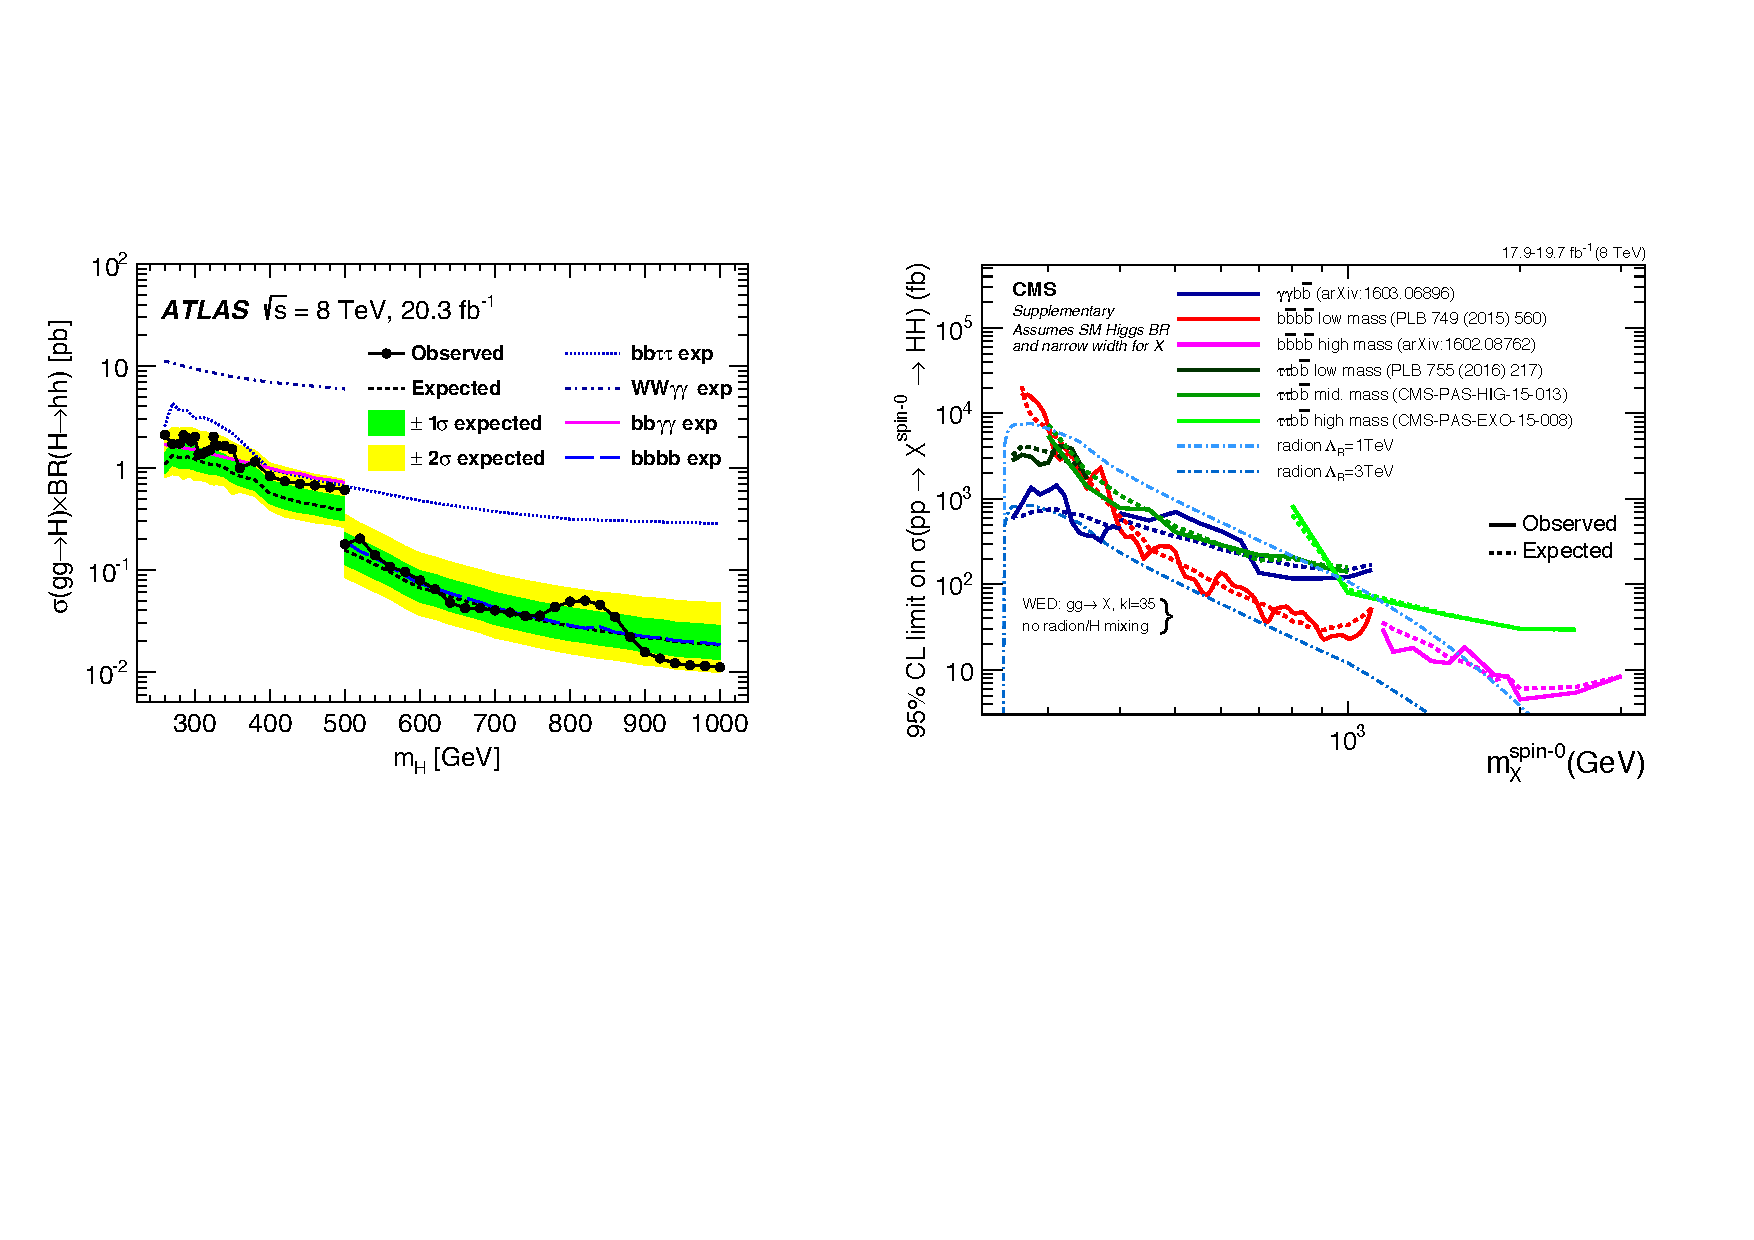
\includegraphics[width=1.0\textwidth, angle=0] {figures/HH_8TeV.pdf}
\caption{(left) ATLAS combination Higgs boson pair production in the $hh\ensuremath{\rightarrow}bb\ensuremath{\tau}\ensuremath{\tau}$, $\ensuremath{\gamma}\ensuremath{\gamma}W{W}^{*}$, $\ensuremath{\gamma}\ensuremath{\gamma}bb$, $bbbb$ channels with $8\,TeV$ data, (right) CMS Observed and expected 95\% CL upper limits on the product of cross section and the branching fraction $\sigma(gg\rightarrow X) \times B(X\rightarrow hh)$ obtained by different analyses assuming spin-0 hypothesis.}
\label{fig:HH_8TeV_Results}   
\end{figure}
%%

\subsection{$H\rightarrow hh \rightarrow bbbb$ channel}
The Higgs boson decay mode in b quarks has the highest branching ratio, this imply that a Di-Higgs final state, with each Higgs dacaying into a b pair, it's the most prominent one between the others. Although search of this kind of final state should take into account the overwhelming multi-jet background, largely produced at hadrons collider.

ATLAS and CMS collaborations analysis scan a mass range $260\, GeV \, < m_{H}  <  3000 \, GeV$, particularly CMS cover from $260\, GeV$ to $1200\, GeV$ and ATLAS from $500\, GeV$ to $3000\, GeV$. Both analysis have different strategy for different $m_H$ ranges: low-mass region ($260\, GeV \, < m_{H}  <  400 \, GeV$), medium-mass ragion ($400\, GeV \, < m_{H}  <  1200 \, GeV$), boosted region ($1200\, GeV \, < m_{H}  <  3000 \, GeV$). The categorisation is chosen to maximise to significance of the analysis. 

The results are shown in figure \ref{fig:HH_bbbb}.
 %%
\begin{figure}[htb]
\centering
	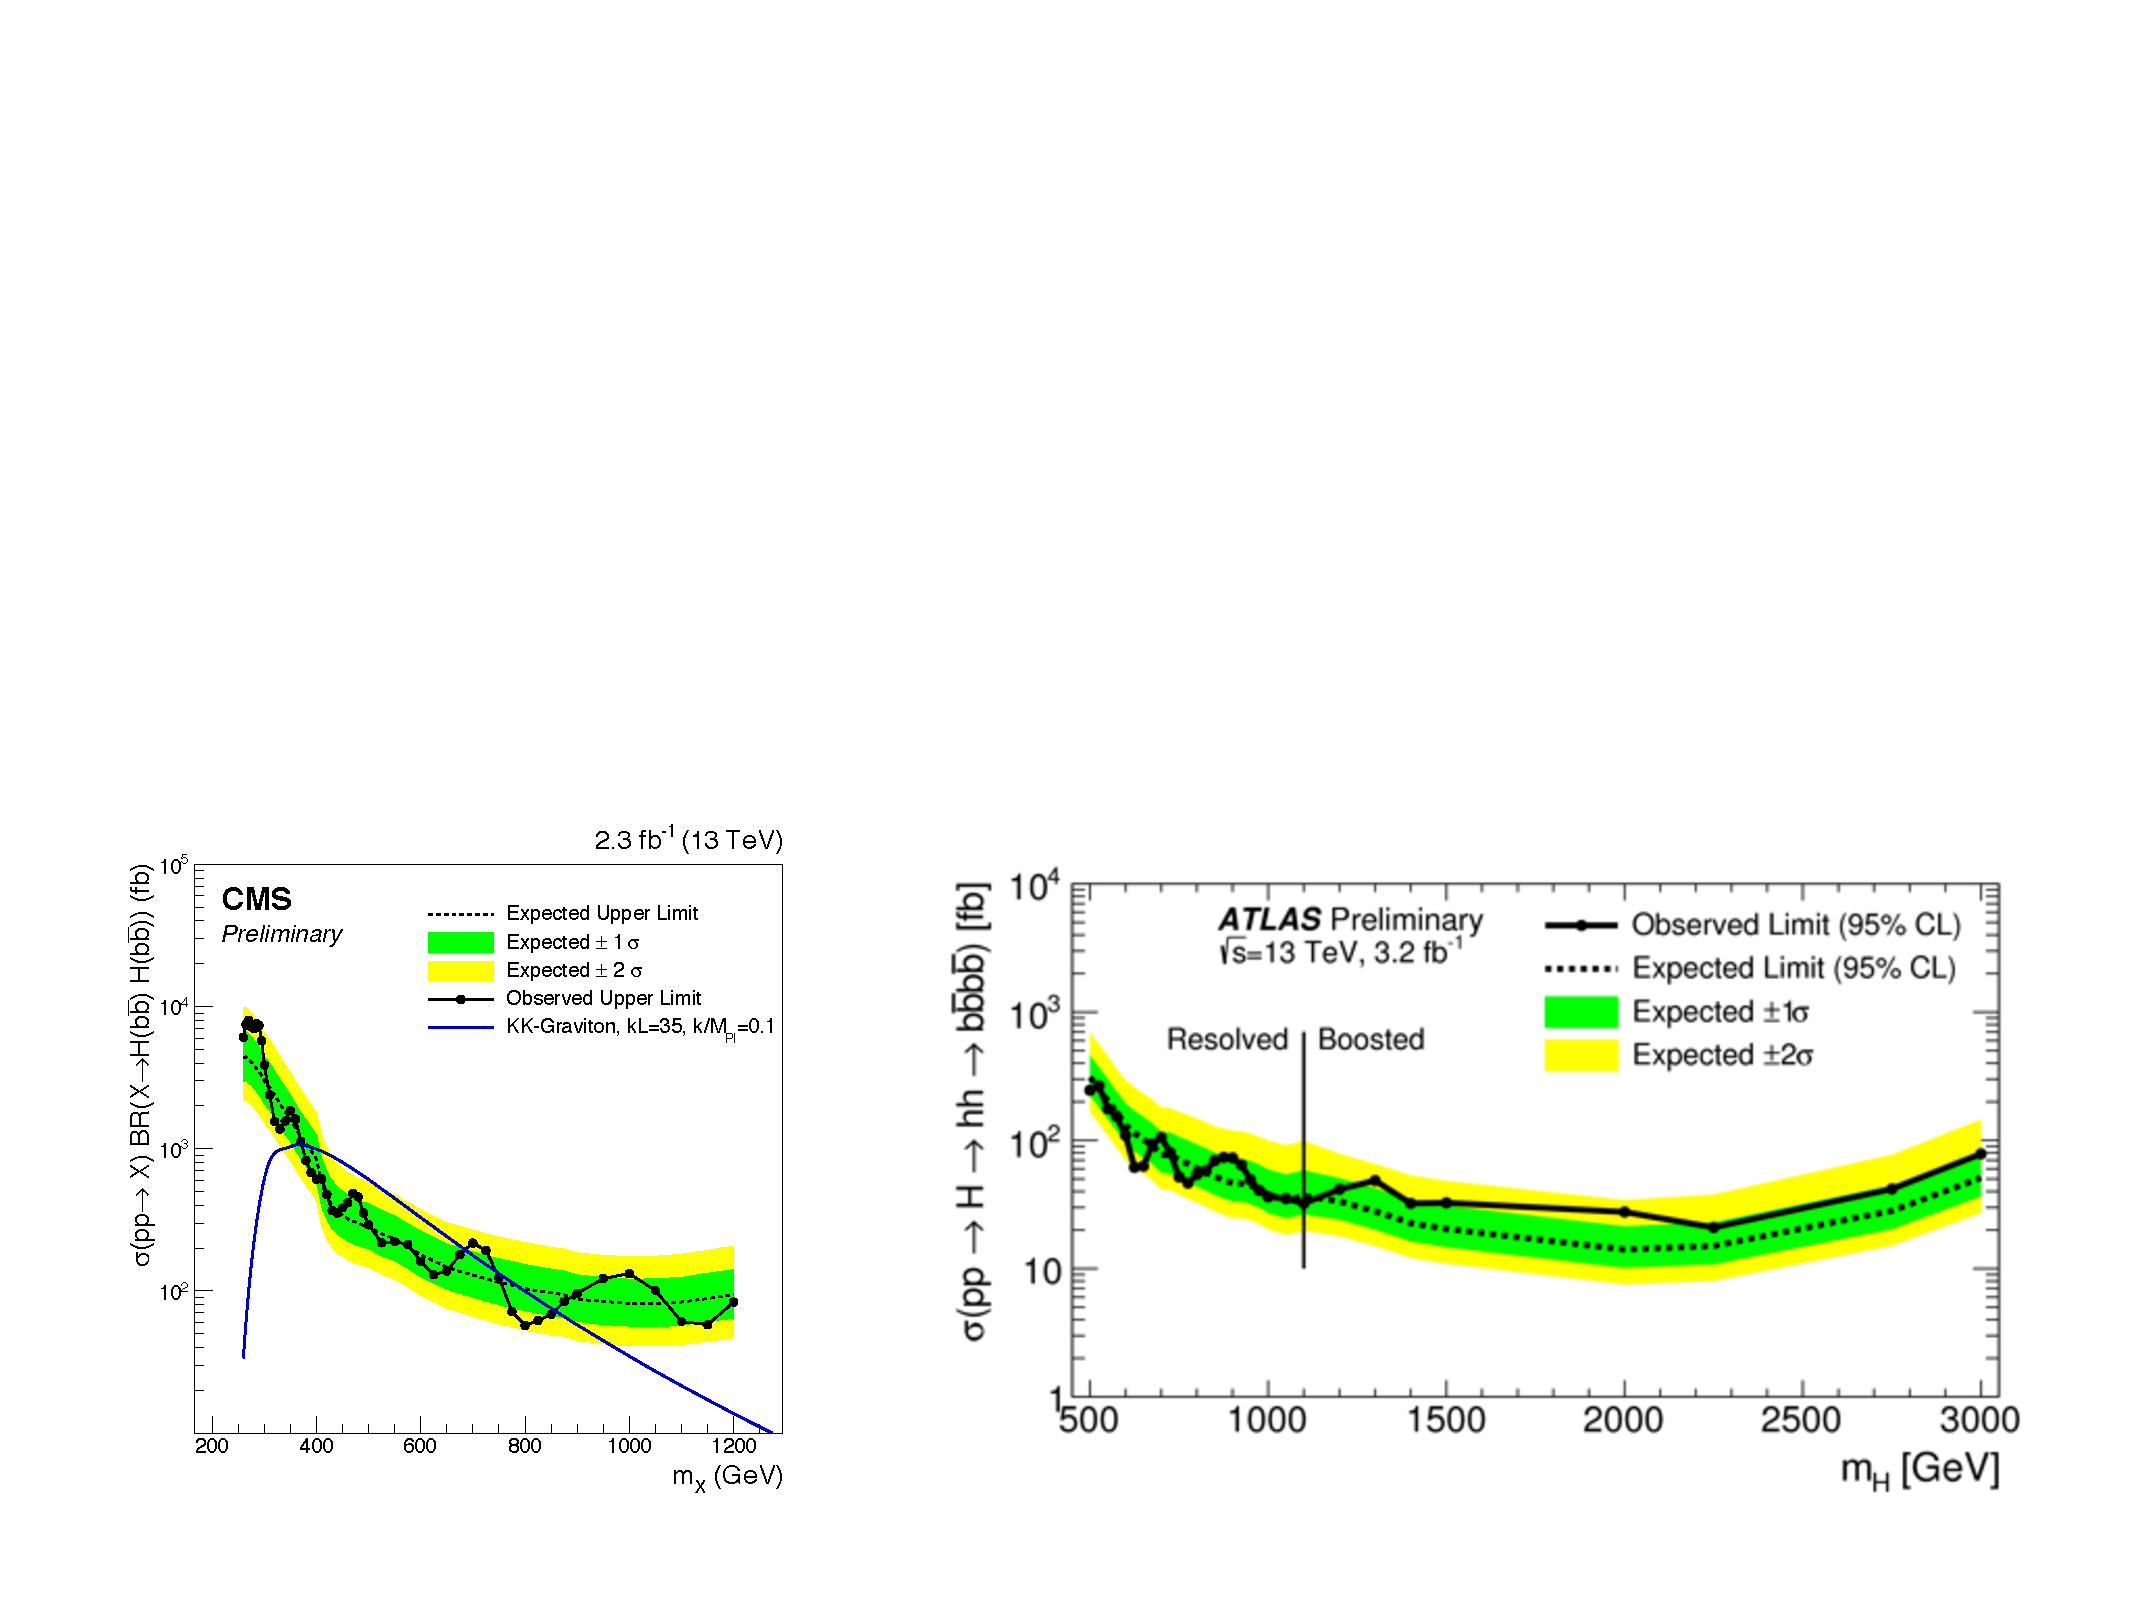
\includegraphics[width=1.0\textwidth, angle=0] {figures/HH_bbbb.pdf}
\caption{(left) CMS: The observed and expected upper limits on the cross section for a spin-2 resonance
$H\rightarrow hh\rightarrow bbbb$ at a 95\% confidence level using data corresponding to an integrated luminosity
of $2.3 fb^{?1}$ at $13 TeV$ using the asymptotic $CL_S$ method, (right) ATLAS: The expected and observed upper limit for $pp\rightarrow H\rightarrow hh\rightarrow bbbb$ with fixed $\Gamma_H = 1 GeV$, at the 95\% confidence level .}
\label{fig:HH_bbbb}   
\end{figure}
%%
 
\subsection{$H\rightarrow hh \rightarrow bb\tau\tau$ channel}
The $bb\tau\tau$ channel can exploit the presence of the $\tau$ leptons to take care of the multi-jet background.

The analysis performed by CMS collaboration scans a $260\, GeV \, < m_{H}  <  900 \, GeV$ and combine three different $\tau\tau$ final state: $\mu\tau_h$, $e\tau_h$ and $\tau_h\tau_h$, where $\tau_h$ stands for the hadronic decays of a $\tau$. 
The finale $m_H$ shape is constructed using a dedicated kinematic fit procedure.

Observed and expected 95\% CL upper limits are shown in figure \ref{fig:HH_bbtt}.


 %%
\begin{figure}[htb]
\centering
	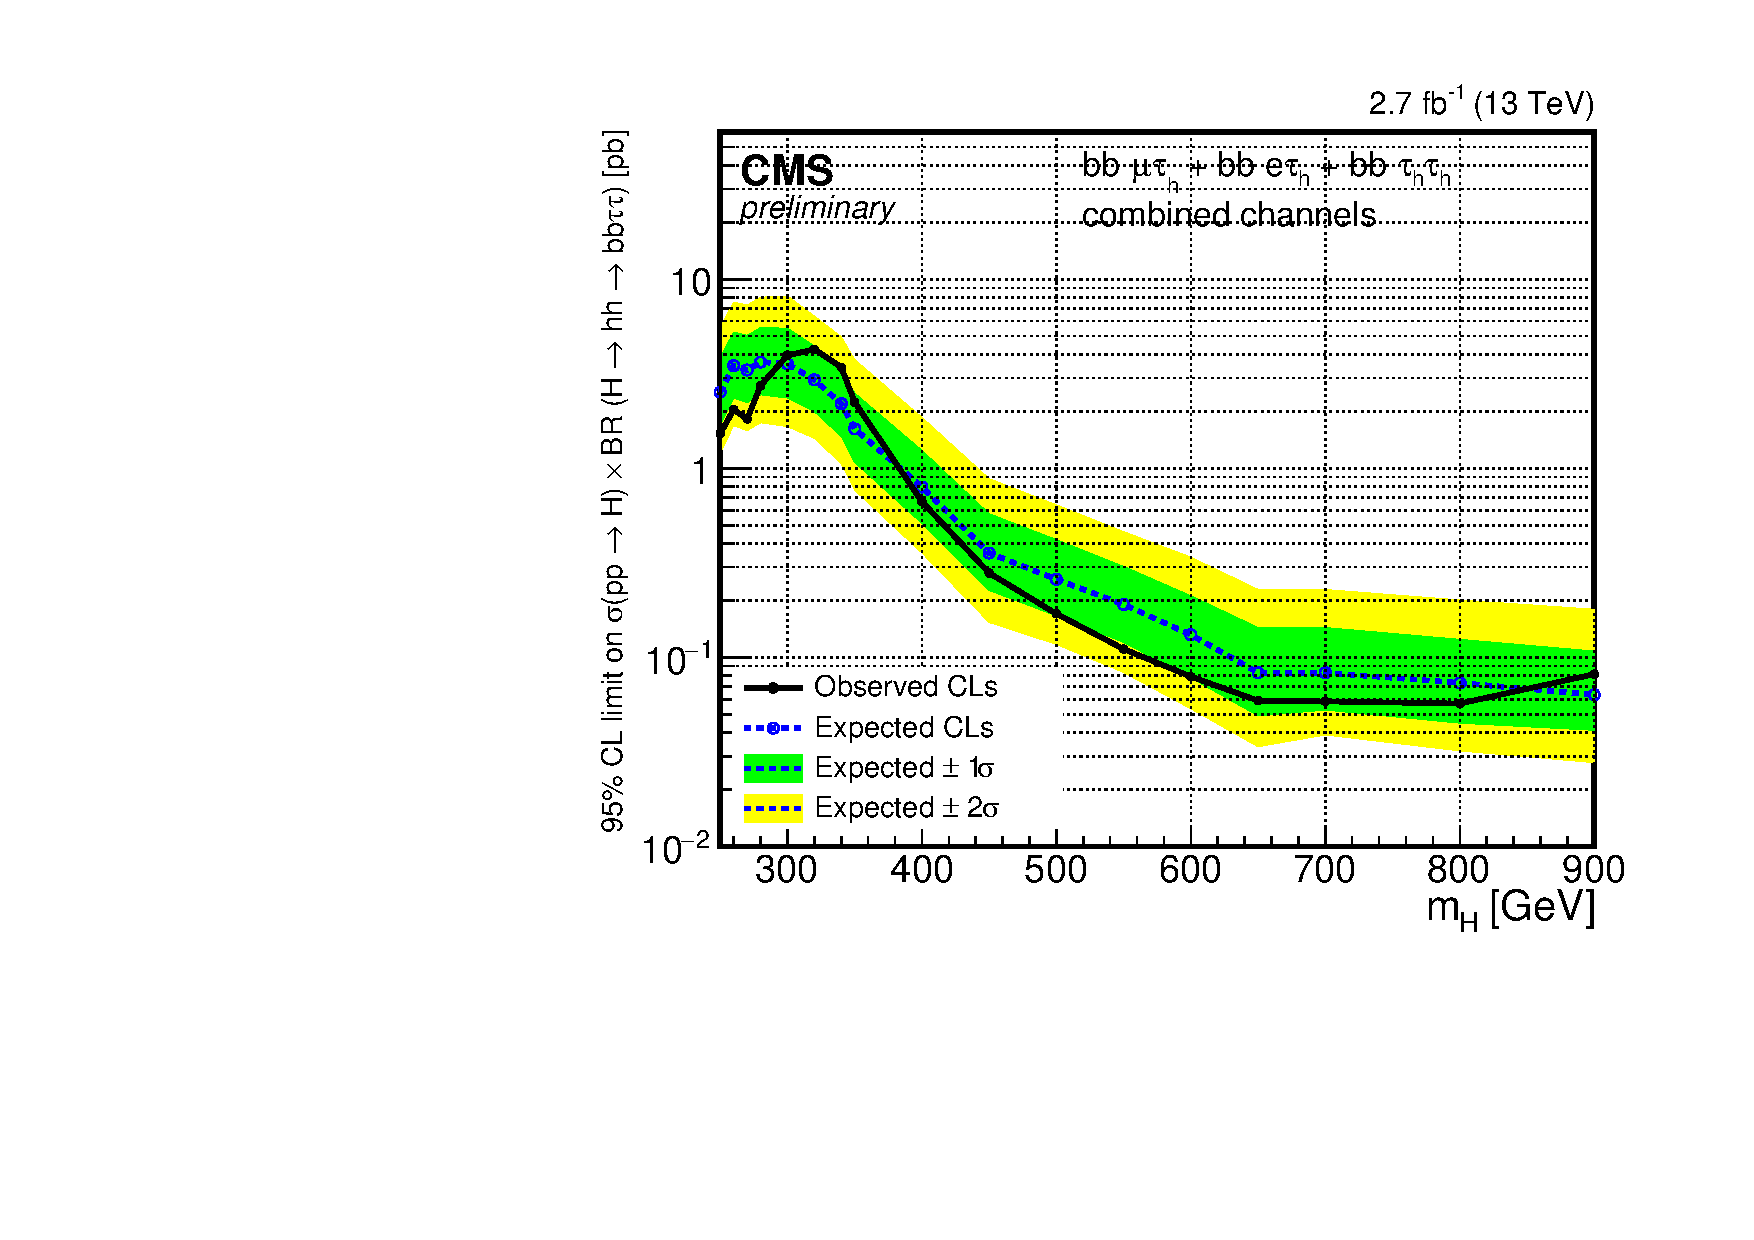
\includegraphics[width=0.7\textwidth, angle=0] {figures/H_hh_bbtautau_CMS_BR.pdf}
\caption{Observed and expected 95\% CL upper limits on $\sigma(pp\rightarrow H) \times BR(H \rightarrow hh \rightarrow bb\tau\tau)$
from the combination of the three channels as a function of the mass of the resonance $m_H$}
\label{fig:HH_bbtt}   
\end{figure}
%%

\subsection{$H\rightarrow hh \rightarrow bbWW$ channel}
The search for resonant Higgs pair production, $H \rightarrow hh$, where one of the h decays as $h\rightarrow bb$, and the other as $H \rightarrow WW \rightarrow l?l?$ (where l is either an electron or a muon) is performed by CMS collaboration using LHC proton-proton collision data at $13\, TeV$. The analysis focuses on the invariant mass distribution of the b-jet pair, searching for a resonant-like excess compatible with the h boson mass in combination with a boosted decision tree discriminant based on kinematic information. The dominant background is tt production with smaller contributions
from Drell-Yan and single top processes. Figure \ref{fig:HH_bbWW} shows the result obtained.

 %%
\begin{figure}[htb]
\centering
	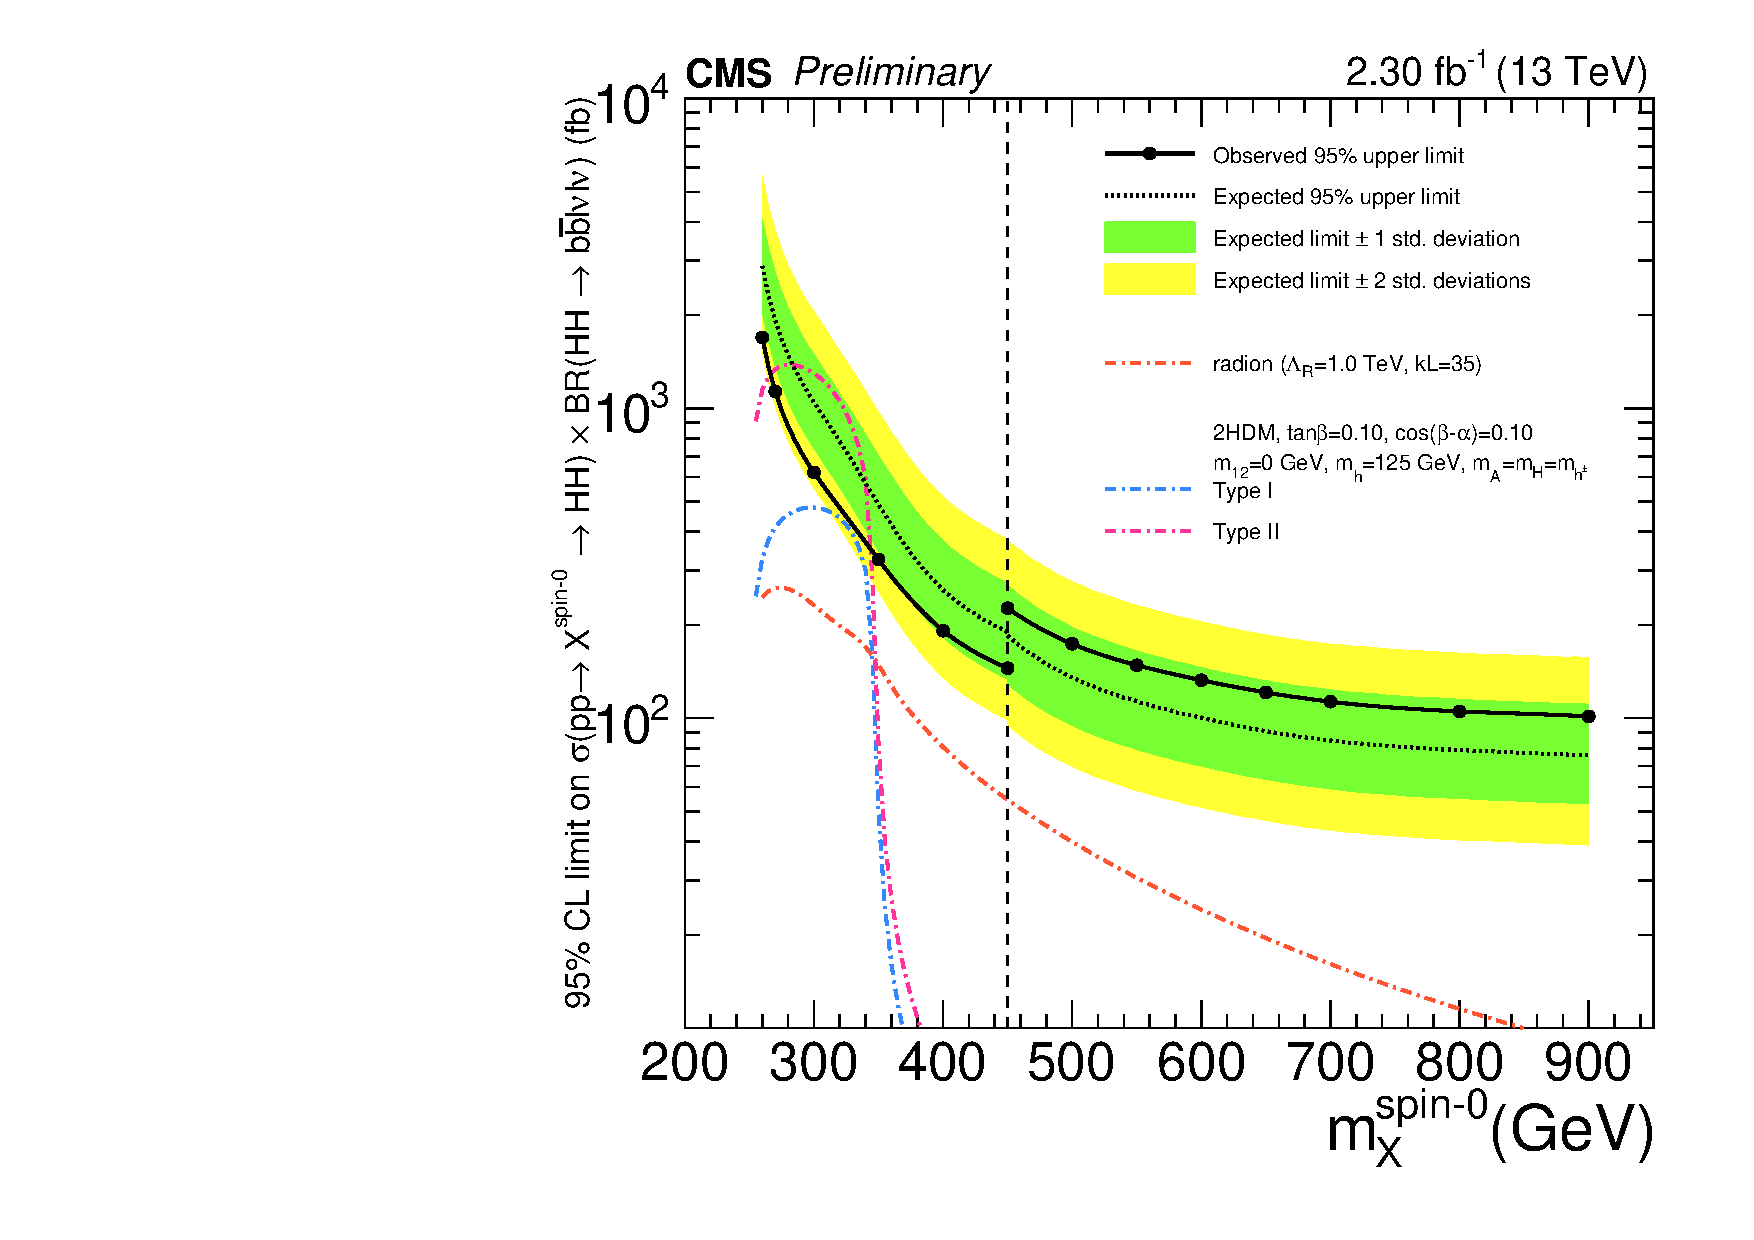
\includegraphics[width=0.6\textwidth, angle=0] {figures/H_hh_bbWW_CMS_BR.pdf}
\caption{Observed and expected 95\% CL upper limits on $\sigma(pp\rightarrow H) \times BR(H \rightarrow hh \rightarrow bbl\nu l\nu)$}
\label{fig:HH_bbWW}   
\end{figure}
%%

\subsection{$H\rightarrow hh \rightarrow bb\gamma\gamma$ channel}

The $bb\gamma\gamma$ final state is particularly promising for the DiHiggs search, as it benefits from the large branching fraction of the $h\rightarrow bb$ decay and the clean di-photon signal, due to high $m_{\gamma\gamma}$ resolution, on top of a smooth continuum di-photon background from multi-jet and multi-photon SM processes. 

The analysis performed by ATLAS collaboration scans masses in the range $275 GeV < m_H < 400 GeV$. A counting approach is adopted in order to estimate the number of signal and background events.

Observed and expected 95\% CL upper limits are shown in figure \ref{fig:HH_bbgg}.
 %%
\begin{figure}[htb]
\centering
	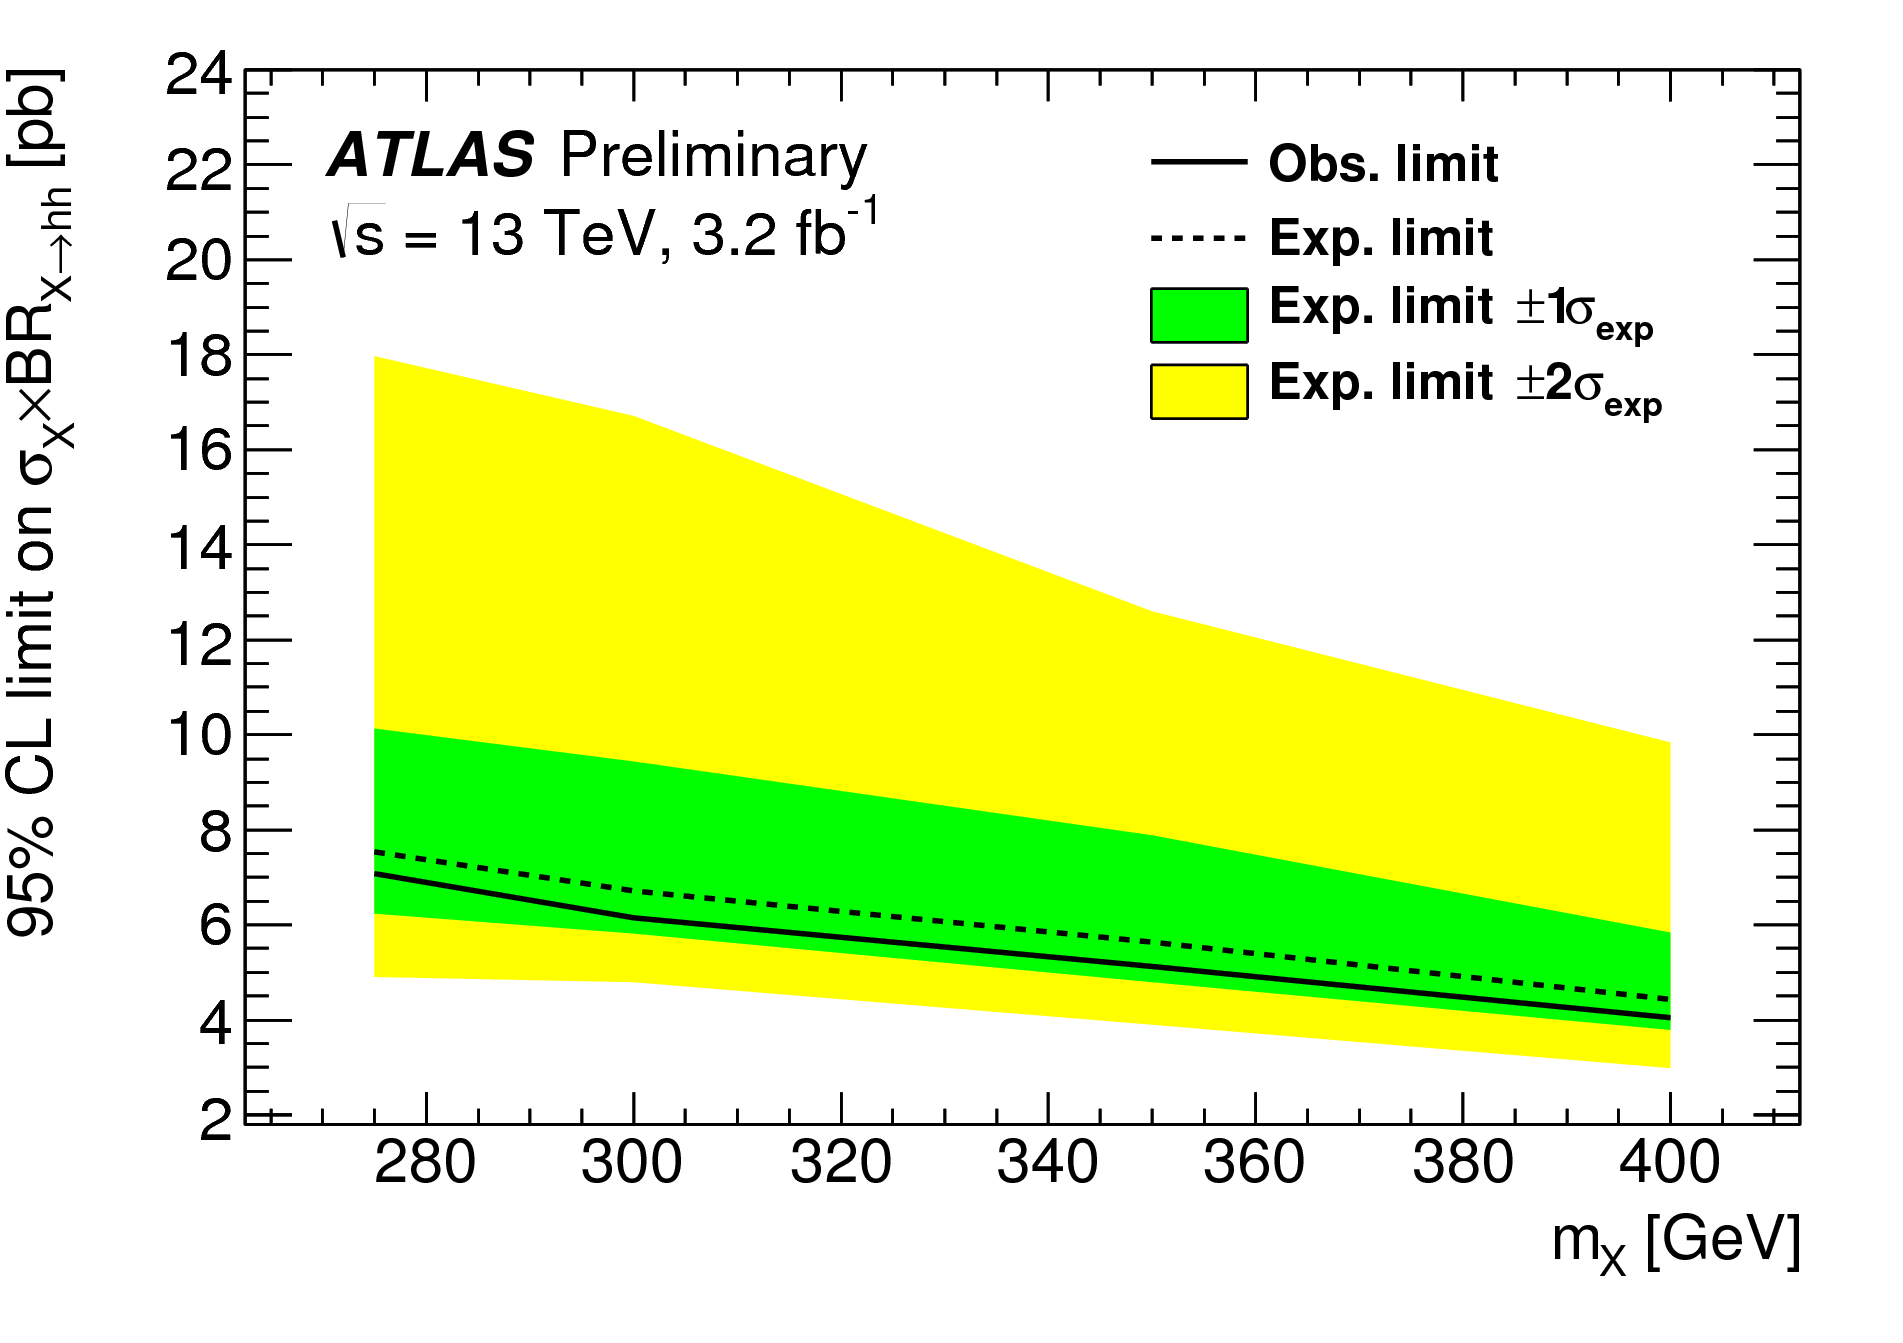
\includegraphics[width=0.6\textwidth, angle=0] {figures/H_hh_bbgg_ATLAS_BR.png}
\caption{Observed and expected 95\% CL upper limits on $\sigma(pp\rightarrow H) \times BR(H \rightarrow hh \rightarrow bb\gamma\gamma)$}
\label{fig:HH_bbgg}   
\end{figure}
%%





